\documentclass[nynorsk,12pt,a4paper]{article}
\usepackage[utf8]{inputenc}
\usepackage{graphicx}
\usepackage{babel}
\usepackage[final]{pdfpages}
\renewcommand*{\familydefault}{\rmdefault}
\title{Visjonsdokument\\
Dynamisk Nettverksbrannmur
}
\author{Espen Gjærde \and Svein Ove Undal}
\date{11.04.2013}

\pagenumbering{arabic}
\begin{document}
\maketitle
\newpage

\section*{Revisjonshistorie}

\begin{table}[h!]
	\begin{tabular}{ l c l r }
	\centering
		\textsc{Dato} & \textsc{Versjon} & \textsc{Forklaring} & \textsc{Forfattar} \\
		\hline 
		01.02.2013 & 1.0 & Dokumentet oppretta & Espen, Svein \\ 
		15.02.2013 & 1.0 & Dokument klar for revisjon & Espen, Svein \\ 
		09.04.2013 & 1.1 & Tabellar oppdatert, små rettingar & Espen \\ 
		11.04.2013 & 2.0 & Oppdatert mtp. django & Espen \\
		16.04.2013 & 2.1 & Kost/Nytte-analyse oppdatert & Espen, Svein\\
		\hline
	\end{tabular}
\end{table}

\newpage
\tableofcontents{}

\newpage

\section{Innleiing}
\paragraph{}
Dette dokumentet er ei analyse av prosjektet som skal gjennomførast, med mål om å avgjere om prosjektet bør startast. Vi vil i dokumentet gå gjennom bakgrunn og mål for prosjektet, greie ut om interessentar og utføre kost/nytte og risikoanalyse. Vi vil også gå gjennom teknologival, standardar for gjennomføring og suksessfaktorar.

\newpage
\section{Bakgrunn for prosjektet}
\paragraph{}
Prosjektet er ei bacheloroppgåve for Espen Gjærde og Svein Ove Undal. Begge studentar ved Avdeling for Informatikk og e-Læring ved \ Høgskolen i Sør-Trøndelag. Prosjektet går ut på å lage ein smart brannmur basert på pålogging via web. Etter dette skal brukaren få tilpassa reglar for sin bruker. 

\subsection{Skildring av problem og behov}
\paragraph{}
For administratorar av nettverk med mange brukarar -- og mange forskjellige typar brukarar -- kan det være vanskeleg å halde oversikt over nettilgang \ og effektivt og rettferdig fordele bandbredde og tilgangar mellom brukarane. Spesielt gjeld dette midlertidige nettverk - tildømes dataparty, eller trådlause gjestenett. Vi tek sikte på å lage eit system som sikrar rettferdig og dynamisk deling av bandbredde, samstundes som det gir rom for å spesialisere reglar for den enkelte brukar. 

\subsection{Skildring av dagens system og rutiner}
\paragraph{}
Det finnast i dag døme på system der brukarar må logge inn for å nytte seg av ressursar. Dette er gjerne måten adgangskontroll for trådlausnett vert gjort på på flyplassar og hotell. Dette er det som blir kalla captive-portal\footnote{\ Captive{}-Portal: System som tvingar brukarar via ei bestemt nettside eller gjennom eitt spesielt punkt. }. Problemet med slike løysingar er at det enten er fritt fram etter du har logga inn, eller at kapasiteten blir delt etter eit <<one-size-fits-all>>-prinsipp. Systema har og veikskapar som macadresse-spoofing \footnote{forfalsking av unik  adresse eller identifikasjon} og DNS-tunnel som ein måte å unngå autentifiseringa heilt.

\newpage
\section{Prosjektmål}
\paragraph{}
Overordna prosjektmål
\begin{itemize}
	\item lage eit effektivt brannmursystem som er enkelt å nytte seg av
	\item tileigne oss meir erfaring og kompetanse
	\item lage eit solid og stabilt sluttprodukt
\end{itemize}

\paragraph{}
For å beskrive måla med prosjektoppgåva er det hensiktsmessig å dele måla inn i føljande kategoriar:
\begin{description}
	\item[Effektmål] --- skildrar effekten sluttbrukar får av å bruke systemet
	\item[Resultatmål] --- skildrar kva som skal ligge føre når prosjektet er ferdig
	\item[Prossessmål] --- mål utviklarane har med å delta i prosessen
\end{description}

\subsection{Effektmål}
\begin{itemize}
	\item Enklare administrasjon av brukarar i mellombels nett
	\item Dynamiske brannmurreglar og enkel administrering av desse
\end{itemize}

\subsection{Resultatmål}
\begin{itemize}
	\item Eit fullverdig brannmursystem med pålogging
	\item Ein fungerande brannmur med individuelle reglar for kvar brukar eller gruppe
	\item Eit enkelt og oversiktleg administrasjonsystem for brannmuren.
	\item Eit system som sjekkar nettverkskonfigurasjon for pålogga maskiner.
	\item Ein pakke med enkel installasjon - gjerne .deb eller tar.gz.
\end{itemize}

\subsection{Prosessmål}
\begin{itemize}
	\item Vidareutvikle kunnskapar om linux og nettverstryggleik
	\item Erfaring med utvikling i Python
	\item Utvikling av eit open source distribuert system
\end{itemize}

\subsection{Omfang}
\begin{itemize}
	\item Det skal vere alternativ å lage informasjon som filer, eller i ein database
	\item Det skal implementerast eit oversiktlig administrasjonspanel
	\item Prosjektet skal være ferdigstilt innan 25.mai 2013.
	\item Systemet blir utvikla og testa for Debian 6.0.6 "Squeeze"
\end{itemize}

\subsection{Prosjektets milepælar og hovudaktivitetar}

\subsubsection{Dokumentasjon}
\begin{table}[h!]
	\centering
	\begin{tabular}{ l l } 
		\textsc{Dato} & \textsc{Milepæl} \\ \hline
		04.02.2013 & Oppstart av prosjektet \\ 
		15.02.2013 & Visjonsdokument til revisjon	\\ 
		10.04.2013 & Kravdokument til revisjon	\\ 
		01.04.2013 & Arkitekturdokument til revisjon \\ 
		25.05.2013 & Sluttrapport ferdig og levert	\\ 
		\hline
	\end{tabular}
\end{table}

\subsubsection{Utviklingsteg / Mål}
\begin{table}[h!]
	\centering
	\begin{tabular}{ l l }
		\textsc{Dato} & \textsc{Milepæl} \\ \hline
		15.02.2013 & Captive-Portal i funksjon \\ 
		20.02.2013 & Brannmur og pålogging styrt av Python	\\ 
		08.03.2013 & Prototype klar til test på TIHLDE-LAN \\ 
		01.04.2013 & Administrasjonspanel i testversjon \\ 
		01.05.2013 & Release Candidate 1 klar	\\ 
		\hline
	\end{tabular}
\end{table}

\subsection{Teknologi}
\paragraph{}
Vi vil basere prosjektet på eksisterande teknologi og programmer med open kjeldekode. Vi vil utvikle systemet i Debian Linux, men systemet skal kunne kjøre på alle linuxplattformer. Mykje av dei programma vi nyttar finnast også til andre *nix-system, og burde med enkle steg kunne nyttast her også. Nedanfor vil vi kort grunngi forskjellige val av teknologi. 
\paragraph{Debian Linux Wheezy}
Debian er den Linuxdistibusjonen med open kjeldekode som er sikrast og mest utbreidd. Det gjere Debian som eit lett val til vårt prosjekt. I tillegg til dette er Debian den linuxversjonen vi har mest erfaring med.
\paragraph{Python}
Som kodespråk mot systemet nyttar vi oss av Python. Slik får vi eit abstraksjonsnivå mellom kode og system, som vi ikkje får med bash-script. Dette gjer det også enklare å portere systemet over til andre plattformer enn Debian Linux. 
\paragraph{Django}
Som brukargrensesnitt vil vert rammeverket Django nytta. Dette er eit web-rammeverk som er bygd i Python, og vi kan dermed få direkte tilgang til den koden vi utviklar i sjølve brannmursystemet. Dette gjer det meir effektivt og enklare å knytte saman brukergrensesnittet og det bakanforliggande systemet.
\paragraph{ISC DHCP-server}
Dette er ein av dei mest utbredte dhcp-tjenarane i marknaden, og er den klart mest brukte i linux-verda. Vi finn det naturlig å nytte denne både fordi kjeldekoden er open, og fordi det gjer eventuell interaksjon mellom systemet vi utviklar og eventuelle eksisterande system enklare. 
\paragraph{IPtables}
For sjølve brannmuren vil vi nytte iptables. Dette er en enkel pakkefiltrerande brannmur som er støtta i dei fleste *nix-systemer. 
\paragraph{Brukardatabase - PAM} 
Vi vil kjøre autentisering gjennom Linux PAM\footnote{\ Pluggable Authentiction Modules: Eit fleksibelt authentiseringsystem. Gir moglegheit for mange forskjellige typar brukardatabasar.}. Dette gjer at sluttbrukar står fritt til å velje brukardatabase. For demonstrasjon og testing vil vi bruke OpenLDAP og FreeRadius som brukardatabasar.

\newpage
\section{Interessentar og rammevilkår}
\subsection{Interessentanalyse}
\begin{table}[h!]
	\begin{tabular}{p{5cm} p{5cm} p{5cm} }
		\textsc{Interessent} & \textsc{Suksesskriterie} & \textsc{Bidrag til prosjektet}\\ \hline \\
		\textbf{Eksterne interessentar} & ~ & ~ \\ 
		Høgskolen i Sør-Trøndelag & Dokumentasjon og kode levert innan frist & Oppdaragsgiver \\ 
		TIHLDE & Programvare stabil under testing & Tilgang til å teste programmet under TIHLDE sitt dataparty. \\ \\
		\textbf{Interne interessentar} & ~ & ~ \\ 
		Studentane & Strukturert jobbing & Systemutviklarar og prosjekteigarar \\ 
		Rettleiar & God kommunikasjon, hyppig oppdatering & Kunnskap, rettleiing  \\ 
	\end{tabular}
\end{table}


\subsection{Rammevilkår}
\begin{itemize}
	\item Produkt og dokumentasjon ferdig innan 25.mai 2013
	\item Produktet skal kunne installerast og brukast av ein brukar utan store krav til linux/nettverks kunnskap.
	\item Systemet er utvikla og testa i Debian 6.0.6 “Wheezy”
	\item Utviklingsmetoden Unified Process vert nytta.
	\item Systemet vert basert på og utgitt som open kjeldekode. 
\end{itemize}

\newpage
\section{Kritiske suksessfaktorar}
\subsection{Suksessfaktorar}
\paragraph{}
Saumlaust system, som fungerer uten at sluttbrukar merker at systemet er der. Systemet skal effektivt gjere nettverket betre å bruke med tanke på ping og yting under stress. 
\paragraph{}
Systemet skal vere særdeles lett å settast opp, det skal ikkje krevst høge kunnskapar innan linux og nettverksadministrasjon for å få systemet til å fungere.

\subsection{Informasjonsbehov}
\paragraph{}
Rettleiar skal haldast oppdatert om framgangen i prosjektet

\newpage
\section{Risikoanalyse}
\begin{description}
	\item[A] Langvarig sjukdom/fråvær av gruppemedlemmer
	\item[B] Samarbeidsvanskar i teamet
	\item[C] Feil på programvare vi er avhengig av
	\item[D] Produkt ikkje i kjørbar versjon ved testtid
	\item[E] Programvare oppfører seg ikkje som forutsett
	\item[F] Vanskeleg brukargrensesnitt
	\item[G] For høge systemkrav
	\item[H] Tap av viktig data
\end{description}
\paragraph{}
Sjå Vedlegg A for risikoscore og utrekning av sannsyn og konsekvens

\begin{figure}[h!]
	\centering
	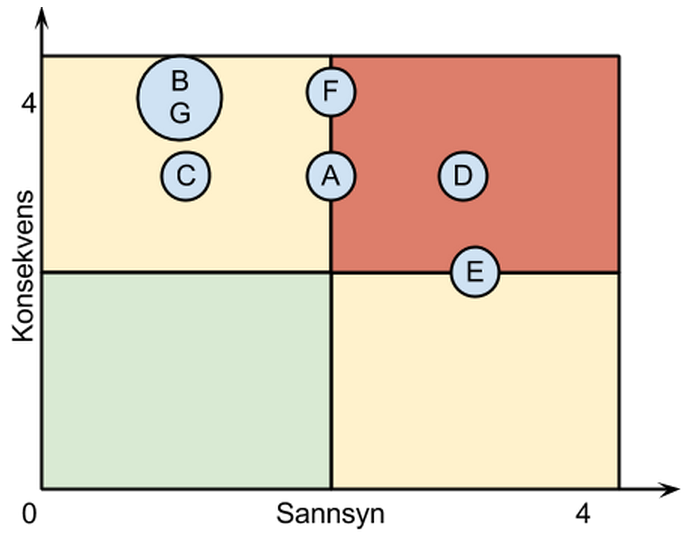
\includegraphics[scale=0.55]{./vdok-img/ros_v2.png}
	\caption{Identifiserte risikoar plassert i koordinatsystem.}
\end{figure}

\newpage
\section{Kost/nytte-analyse}
\paragraph{}
Dette er eit bachelorprosjekt som baserer seg på bruk av open kjeldekode og alle nytta verktøy er opne og fritt tilgjengeleg. All kjeldekode vil også verte publisert under ein open lisens. Det er derfor vanskeleg å sette opp gode kostnadsvurderingar; arbeidskraft, materia og verkty er gratis. Likevell vert det sett opp ei kost/nytte-analyse der ein tek utgangspunkt i sal av nettilgang. 

\subsubsection{Kvantifiserbar nytte}
\paragraph{Mindre bruk av eksterne konsulentar}
Systemet let seg lett administrere via eit nettbasert brukargrensesnitt, og vi kan derfor medrekne mykje mindre bruk av konsulentar. Å vedlikehalde og justere ein brannmur og eit tilgangsystem er mykje arbeid. Vi reknar med 10 timar i månaden, altså 120 timar pr år. Ved å gå over til dette systemet, som er enkelt å administrere kan vi spare inn halvparten av dette, då dei avanserte innstillingane i brannmuren justerer seg sjølv -- ut i frå tilgjengeleg kapasitet. 
\paragraph{Betre utnytting av nettlinje}
Ved at dette systemet automatisk lastbalanserer den ledige kapasiteten mellom brukarane i nettverket, kan fleire brukarar bruke same linja. Systemet sikrar at ingen kan "stele" linja og brukaropplevinga vil bli betre. Brukartalet skal kunne aukast med 25\% på same nettlinje.
\paragraph{Auka sal av nettilgang}
I tillegg til dette vert det i kost/nytte-analysa teke utgangspunkt i at systemet vert nytta ein stad der ein skal selje internett-tilgang. Timepris for tilgang vert da sett til 60kr pr brukar. Vi tek utgangspunkt i at det vert  i snitt seld 60 brukartimar kvar dag, noko som gir ei årsomsetning på (60*365)*60 = 1 314 000 kr. Dette kan vi potensielt auke med 25\% utan å måtte ha dyrare nettlinje. 

\subsubsection{Ikkje-kvantifiserbar nytte}
\begin{itemize}
	\item God kompatibilitet med andre brukardatabasar
	\item Lykkelege brukarar
\end{itemize}
\subsection{Estimerte kostnadar}
\paragraph{Utviklingskostnader}
Prosjektgruppa består av to utviklarar som kvar har 450 timar til disposisjon. Som utgangspunkt for kostnaden vert det rekna med ein timekostnad på 450kr pr utviklar. Utviklingskostnadene er altså 2*450*450 = 405 000 kr
\paragraph{Maskinvare}
Systemet har låge systemkrav, og skal kunne kjørast på ein minipc. Einaste krav er to nettverksportar. Vi har testa systemet på ARM-pcen RaspberryPI\footnote{ http://raspberrypi.org/faqs Sist vitja 16.04.2013} med eit ekstra USB-nettverkskort. Kostnaden for dette utstyret er berre 350kr, men ein må og rekne med litt ekstrautstyr.
\begin{table}[h!]
	\centering
	\begin{tabular}{l r}
	\textsc{Utstyr} & 	\textsc{NOK} \\ \hline
	Raspberry PI	& 	350 \\
	Min 4GB Lagring	&	100	\\
	Kabinett		&	100	\\
	Straumforsyning	&	200	\\
	Ekstra nettverkskort & 	200 \\
	I/O-utstyr		&	400	\\ \hline
	\textbf{Total}	&	1450 \\ \hline \hline
	\end{tabular}
	\caption{Estimerte prisar på maskinvareutstyr}
\end{table}


\subsection{Samanstilling av kostnadar og nytte}
\begin{table}[h!]
	\centering
	\begin{tabular}{l r r r}
	\textsc{Forklaring} & \textsc{1.år} & \textsc{2.år} & \textsc{Total} \\ \hline
	Lågare vedlikehaldskostnad & 30 000 & 30 000 & 60 000 \\
	Auka salsinntekter & 328 500 & 328 500 & 657 000 \\
	Maskinvare & - 1 450 & ~ & - 1 450 \\
	Utviklingskostnader & - 404 550 & ~ & - 405 000 \\ \hline
	\textbf{Total} & ~ & ~ & \textbf{252 550} \\ \hline \hline
	\end{tabular}
	\caption{Samenstilling av kost vs. nytte}
\end{table}
\newpage
\section{Retningslinjer og standardar}
\subsection{Krav til dokumentasjon}
\paragraph{}
Endeleg versjon av følgjande dokumentasjon skal være klar 5.mai:
\begin{itemize}
	\item Visjonsdokument
	\item Kravdokument
	\item Arkitekturdokument
\end{itemize}
\paragraph{}
Vidare skal følgjande dokumentasjon foreligge ved prosjektinnlevering:
\begin{itemize}
	\item Brukardokumentasjon
	\item Installasjonsrettleiing
	\item Sluttrapport
\end{itemize}

\subsubsection{Utforming og digitale format}
\paragraph{}
Følgjande krav vert sett til levert dokumentasjon
\begin{itemize}
	\item Dokumentasjonen vert utforma i \LaTeX
	\item Dokumentasjon vert tilgjengeleg i PDF-format
	\item Framsida av sluttrapporten skal være etter mal frå HiST Avdeling for Informatikk og e-Læring
\end{itemize}

\subsection{Krav til kvalitetskontroll}
\paragraph{}
Kvalitetsgjennomgang blir tildels dekka av dei daglege utviklingsmøta i prosjektgruppa. Vi får her tilbakemeldingar om eventuelle endringa som burde vore utført, og om det må føyast til noko. 

\paragraph{}
Prosjektgruppa må også ha en gjennom gang av følgjande:
\begin{itemize}	
	\item Pythonkode
	\item Django / HTML-kode
	\item Brukarvennligheit på nettsida
	\item Databasestruktur og tryggleik
\end{itemize}

\paragraph{}
I tillegg til å kvalitetsikre, testar vi programvara undervegs og etter kvar endring. Testinga undervegs blir ein peikepinne på om systemet fungerer som det skal, samt at vi utbetrar alle problema når dei oppstår. Vi vil òg ha ei utbredt testing av ein prototype på TIHLDE{}-lan, som vil effektivt vise veikskapar og styrkar i systemet.

\subsection{Krav til standardar og metodar}
\paragraph{}
Systemet skal bruke kjent teknologi og basere seg på innførte standardar. Dette fordi det for sluttbrukar sine klientar ikkje skal være behov for spesialutstyr eller eigne klientprogram. 

\subsubsection{Programmeringstandardar}
\begin{itemize}
	\item Programmering skjer i språka HTML og Python.
	\item Alle metodar skal ha engelske navn, og følge kjente namnekonvensjonar i sine respektive språk.
	\item Kommentarar og forklaringar i kodefilene skal skrivast på engelsk.
\end{itemize}

\subsubsection{Konfigurasjonsfiler}
\begin{itemize}
	\item Konfigurasjonsfiler og programvare skal i størst mulig grad følge standardar og ligge der det er naturlig i eit linux / Debian{}-system.
	\item Kommentarar og forklaringar i filene skal skrivast på engelsk
\end{itemize}

\subsubsection{Bruk av verktøy}
\begin{itemize}
	\item Versjonskontroll skjer med versjonshandteringssystemet GIT. 
	\item Systemet blir testa på ei tjenermaskin med operativsystemet Debian 6.0.6 <<Squeeze>>. 
\end{itemize}
\subsubsection{Andre standardar}
\begin{itemize}
	\item Systemet skal baserast på kjente og de{}-facto standardprotokollar som IP, TCP, DHCP og HTTP.
	\item Språk for administrasjonsystemet skal være norsk - nynorsk.
\end{itemize}

\subsection{Endringshandtering}
\begin{enumerate}
	\item Eventuell mistanke om problem meldast tidleg til dei andre i prosjektgruppa
	\item Det skal arbeidast med å få oversikt over endringar og ringverknadar.
	\item Endringa dokumenterast og avvik rapporterast
	\item Tidsplanar justerast
	\item Endringa blir gjennomført
	\item Evaluering av endring og endringsprosessen vert gjennomført
\end{enumerate}

\newpage
\section{Prosjektorganisering}
\paragraph{}
Prosjektorganisasjonen består av ei prosjektgruppe, studentane, og rettleiar som også utgjer styringsgruppa.

\begin{figure}[h!]
	\centering
	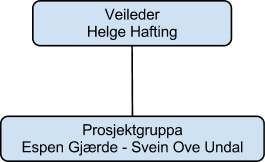
\includegraphics[scale=0.75]{./vdok-img/vdok-org.png}
	\caption{Prosjektorganisasjonen}
\end{figure}

\newpage
\section{Tilråding om vidare arbeid}
\paragraph{}
Med bakgrunn i kost/nytte-analysa og dette visjonsdokumentet elles, vert det tilrådd at prosjektet vert utvikla vidare. 

\newpage

\appendix
\section{ROS-analyse}

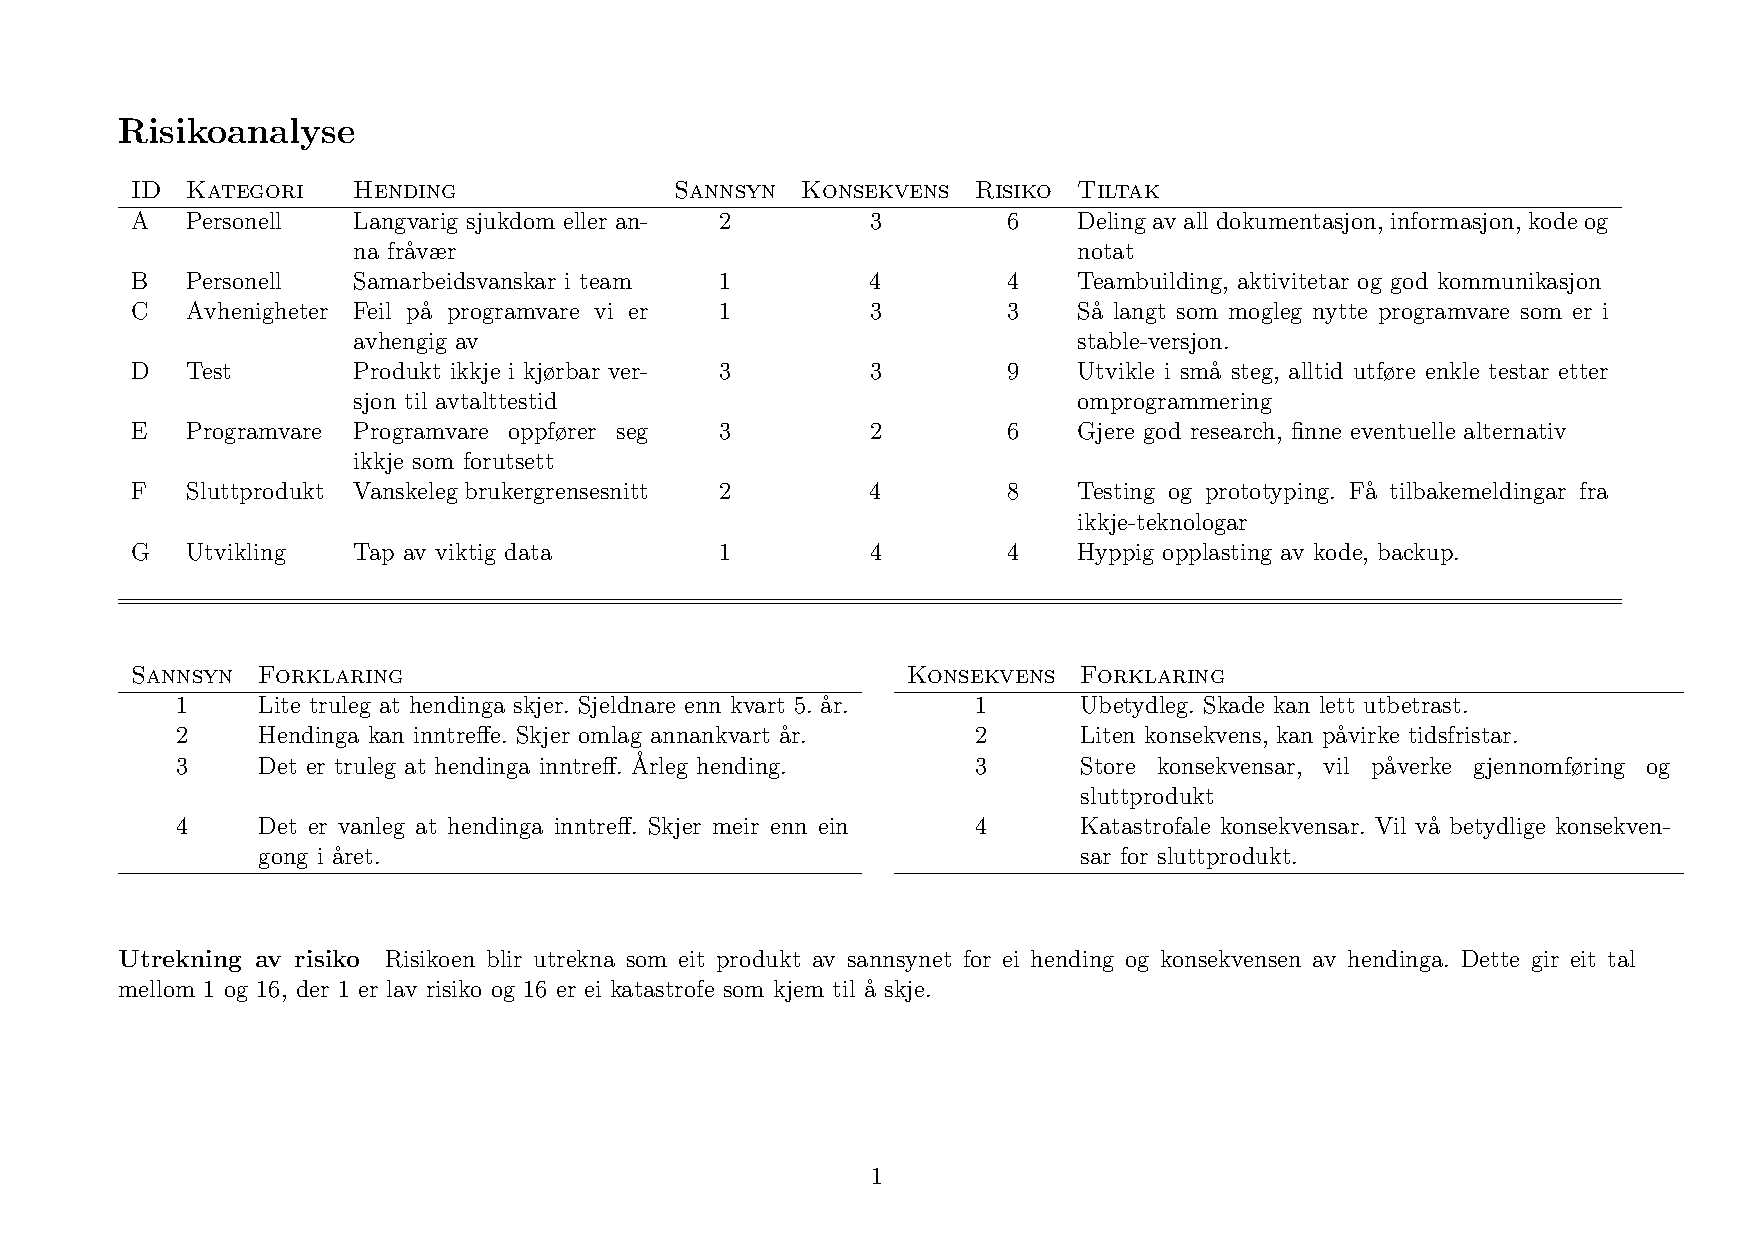
\includepdf[pages=1,landscape]{20E_VDOK_VEDLEGGA_ROS.pdf}

\end{document}











